\chapter{La combustion~: ce dont un feu a besoin}\label{ch:g4:what-a-fire-needs}

Un feu de camp, à la tombée du jour. Il lui a fallu du bois sec, une
allumette pour démarrer, et le vent qui le traverse le garde bien vif.
Au bout d'une heure, les bûches ne sont plus que des braises rougeoyantes
et de la cendre blanche, et une fumée grise s'est envolée dans le ciel.
Où le bois est-il passé~? De quoi un feu a-t-il besoin, et que
laisse-t-il derrière lui~?

\begin{recall}
L'\omterm{def:g4:air-a-mixture-of-gases:air}{air} est un \omterm{def:g2:mixing-and-dissolving:mix}{mélange} de gaz~: environ quatre cinquièmes d'azote et un
cinquième d'oxygène, avec un peu d'argon et de dioxyde de carbone. Une
flamme prend l'oxygène de l'\omterm{def:g4:air-a-mixture-of-gases:air}{air} qui l'entoure~; une bougie sous un bocal
s'éteint quand il reste trop peu d'oxygène
(\cref{ch:g4:air-a-mixture-of-gases}).
\end{recall}

\begin{omfigure}
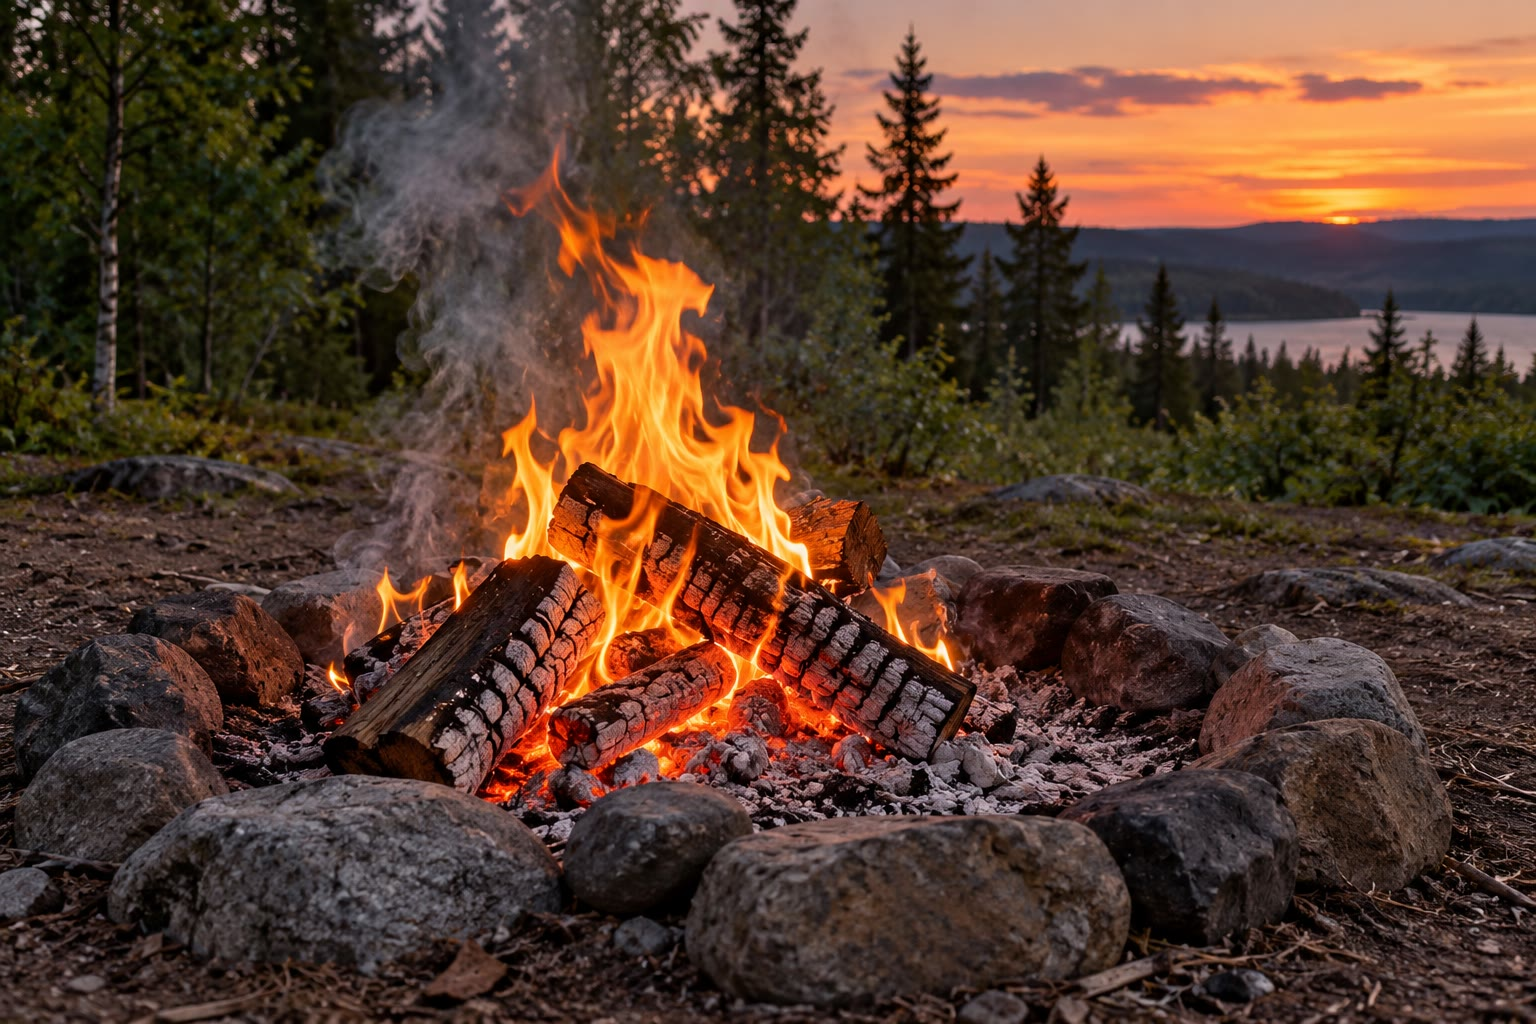
\includegraphics[width=0.6\linewidth]{images/book1/ai/g4-campfire.jpg}

{\small Un feu de camp~: du bois, de l'\omterm{def:g4:air-a-mixture-of-gases:air}{air} et une allumette --- et
ensuite de la cendre et de la fumée.}
\end{omfigure}

\section{Les combustibles}

\begin{definition}[Combustible]\label{def:g4:what-a-fire-needs:fuel}
Un \emph{combustible}\index{combustible} est un matériau qui peut \omterm{def:g4:what-a-fire-needs:burning}{brûler}
en dégageant de la chaleur et de la lumière~: le bois, le papier, le
charbon, la cire de bougie, le gaz d'une cuisinière, l'essence, le fioul.
\end{definition}

\begin{example}[Combustibles solides, liquides et gazeux]\label{ex:g4:what-a-fire-needs:fuels}
Le bois, le papier, le charbon et la cire de bougie sont des
\omterm{def:g4:what-a-fire-needs:fuel}{combustibles} solides. L'essence et le fioul sont des \omterm{def:g4:what-a-fire-needs:fuel}{combustibles}
liquides. Le gaz d'une cuisinière et le gaz d'un briquet sont des
\omterm{def:g4:what-a-fire-needs:fuel}{combustibles} gazeux.
\end{example}

\begin{remark}[Tout ne brûle pas]\label{rem:g4:what-a-fire-needs:not}
La pierre, le sable, le verre et l'eau ne brûlent pas~: ce ne sont pas
des \omterm{def:g4:what-a-fire-needs:fuel}{combustibles}. C'est pourquoi une cheminée est construite en pierre
ou en brique, et pourquoi on utilise le sable et l'eau pour éteindre
les feux.
\end{remark}

\section{Le triangle du feu}

\begin{definition}[Triangle du feu]\label{def:g4:what-a-fire-needs:fire-triangle}
Un feu a besoin de trois choses en même temps~: un \omterm{def:g4:what-a-fire-needs:fuel}{combustible}, de
l'oxygène venu de l'\omterm{def:g4:air-a-mixture-of-gases:air}{air}, et de la chaleur pour démarrer. On représente
ces trois choses comme les trois côtés d'un triangle, le
\emph{triangle du feu}\index{triangle du feu}. S'il manque un côté, il
n'y a pas de feu.
\end{definition}

\begin{omfigure}
\begin{tikzpicture}[font=\small]
  \coordinate (A) at (0,0); \coordinate (B) at (5,0); \coordinate (C) at (2.5,4.1);
  \draw[line width=3pt, brown!70!black] (A) -- (B);
  \draw[line width=3pt, omDef] (B) -- (C);
  \draw[line width=3pt, red!75!black] (C) -- (A);
  \node[below=4pt, font=\small\bfseries, brown!60!black] at (2.5,0) {combustible};
  \node[right=4pt, font=\small\bfseries, omDef] at (3.75,2.05) {oxygène (de l'air)};
  \node[left=4pt, font=\small\bfseries, red!75!black] at (1.25,2.05) {chaleur (pour démarrer)};
  % a flame in the middle
  \fill[orange!80] (2.5,0.55) .. controls (1.95,1.15) and (2.35,1.75) .. (2.55,2.3)
    .. controls (2.75,1.75) and (3.05,1.15) .. (2.5,0.55);
  \fill[yellow!80] (2.5,0.7) .. controls (2.25,1.05) and (2.4,1.35) .. (2.52,1.65)
    .. controls (2.62,1.35) and (2.75,1.05) .. (2.5,0.7);
\end{tikzpicture}

{\small Le \omterm{def:g4:what-a-fire-needs:fire-triangle}{triangle du feu}~: \omterm{def:g4:what-a-fire-needs:fuel}{combustible}, oxygène et chaleur, tous les
trois ensemble.}
\end{omfigure}

\begin{example}[Craquer une allumette]\label{ex:g4:what-a-fire-needs:match}
On frotte la tête d'une allumette sur le côté de sa boîte. Le
frottement la chauffe assez pour qu'elle se mette à \omterm{def:g4:what-a-fire-needs:burning}{brûler}~: c'est le
côté chaleur du triangle. Le bois de l'allumette est le \omterm{def:g4:what-a-fire-needs:fuel}{combustible}, et
l'\omterm{def:g4:air-a-mixture-of-gases:air}{air} apporte l'oxygène.
\end{example}

\begin{example}[Souffler sur des braises]\label{ex:g4:what-a-fire-needs:embers}
Des braises rougeoyantes qui semblent presque éteintes se rallument en
flammes quand quelqu'un souffle dessus~: le souffle apporte plus d'\omterm{def:g4:air-a-mixture-of-gases:air}{air},
donc plus d'oxygène, au \omterm{def:g4:what-a-fire-needs:fuel}{combustible} encore chaud.
\end{example}

\section{Brûler fabrique de nouvelles substances}

\begin{definition}[Brûler, combustion]\label{def:g4:what-a-fire-needs:burning}
Un \omterm{def:g4:what-a-fire-needs:fuel}{combustible} \emph{brûle}\index{bruler@brûler} quand il prend de l'oxygène à
l'\omterm{def:g4:air-a-mixture-of-gases:air}{air} en dégageant de la chaleur et de la lumière. Les chimistes
appellent cela une \emph{combustion}\index{combustion}. Pendant une
combustion, le \omterm{def:g4:what-a-fire-needs:fuel}{combustible} et l'oxygène sont consommés, et de nouvelles
substances apparaissent~: de la fumée, de la cendre, du dioxyde de
carbone et de la vapeur d'eau.
\end{definition}

\begin{proposition}[Une combustion ne peut pas être défaite]\label{prop:g4:what-a-fire-needs:new}
La cendre et la fumée d'un feu ne redeviennent pas du bois, même si
l'on attend très longtemps. \omterm{def:g4:what-a-fire-needs:burning}{Brûler} fabrique de nouvelles substances qui
n'existaient pas avant~; le \omterm{def:g4:what-a-fire-needs:fuel}{combustible} a disparu pour de bon.
\end{proposition}

\begin{inthelab}[Un verre froid au-dessus d'une bougie]
L'enseignant tient un instant un bécher en verre froid et sec, retourné,
au-dessus de la flamme d'une bougie. L'intérieur du verre se couvre de
buée, de minuscules gouttelettes d'eau~: la vapeur d'eau produite par la
bougie qui \omterm{def:g4:what-a-fire-needs:burning}{brûle} est redevenue liquide sur le verre froid. Une bougie
qui \omterm{def:g4:what-a-fire-needs:burning}{brûle} fabrique de l'eau, et aussi du dioxyde de carbone, que l'on
peut mettre en évidence par un test vu dans un chapitre suivant.
\end{inthelab}

\begin{omfigure}
\begin{tikzpicture}[font=\small, scale=1.3]
  % candle
  \fill[white, draw=black!50] (-0.25,0) rectangle (0.25,1.2);
  \draw[black!70] (0,1.2) -- (0,1.33);
  \fill[orange!85] (0,1.3) .. controls (-0.16,1.5) and (-0.06,1.75) .. (0,1.95)
    .. controls (0.06,1.75) and (0.16,1.5) .. (0,1.3);
  \fill[yellow!85] (0,1.36) .. controls (-0.08,1.5) and (-0.03,1.62) .. (0,1.72)
    .. controls (0.03,1.62) and (0.08,1.5) .. (0,1.36);
  % upturned cold beaker above
  \pic[transform shape, rotate=180] at (0,4.3) {beaker={0}{white}};
  \foreach \x/\y in {-0.6/3.9,-0.45/4.1,-0.2/3.95,0.1/4.15,0.35/3.9,0.6/4.05,
                     -0.7/3.5,0.7/3.4,-0.72/3.0,0.72/2.9}
    \fill[omDef!55] (\x,\y) circle (0.035);
  \draw[<-, omProp, thick] (0.68,3.95) -- (2.0,4.2) node[right, text=black]
    {gouttelettes d'eau};
  \draw[<-, omProp, thick] (0.85,3.2) -- (2.0,3.3) node[right, text=black]
    {verre froid, retourné};
  \draw[<-, omProp, thick] (0.15,1.7) -- (2.0,1.9) node[right, text=black]
    {la flamme~: la cire qui brûle};
  \draw[<-, omProp, thick] (0.3,0.6) -- (2.0,0.7) node[right, text=black]
    {la cire~: le combustible};
\end{tikzpicture}

{\small Un verre froid tenu au-dessus d'une bougie se couvre de buée~: la
cire qui \omterm{def:g4:what-a-fire-needs:burning}{brûle} fabrique de la vapeur d'eau.}
\end{omfigure}

\begin{example}[Ce que devient une bûche]\label{ex:g4:what-a-fire-needs:log}
Une bûche de quelques kilogrammes se réduit en brûlant à un petit tas de
cendre. La plus grande partie du bois n'a pas disparu~: avec l'oxygène
de l'\omterm{def:g4:air-a-mixture-of-gases:air}{air}, elle est devenue de la fumée, du dioxyde de carbone et de la
vapeur d'eau, qui sont des gaz et s'en vont dans le ciel.
\end{example}

\section{Éteindre un feu}

\begin{method}[Éteindre un feu~: enlever un côté]\label{met:g4:what-a-fire-needs:out}
Pour éteindre un feu, on enlève un côté du \omterm{def:g4:what-a-fire-needs:fire-triangle}{triangle du feu}~:
\begin{itemize}
  \item \textbf{enlever l'oxygène}~: couvrir le feu avec une couverture
        anti-feu, un couvercle ou du sable, pour que l'\omterm{def:g4:air-a-mixture-of-gases:air}{air} ne puisse plus
        l'atteindre~;
  \item \textbf{enlever la chaleur}~: verser de l'eau sur du bois ou du
        papier qui \omterm{def:g4:what-a-fire-needs:burning}{brûle}, ce qui le refroidit au-dessous du point où il
        peut \omterm{def:g4:what-a-fire-needs:burning}{brûler}~;
  \item \textbf{enlever le \omterm{def:g4:what-a-fire-needs:fuel}{combustible}}~: fermer le robinet du gaz, ou
        débroussailler les plantes sèches autour d'un feu de forêt.
\end{itemize}
\end{method}

\begin{omfigure}
\begin{tikzpicture}[font=\small, scale=0.7]
  \foreach \k/\lab/\side in {0/{une couverture~:\\ plus d'oxygène}/1, 1/{de l'eau~:\\ plus de chaleur}/2,
                              2/{gaz fermé~:\\ plus de combustible}/0} {
    \begin{scope}[xshift=\k*6.2cm]
      \coordinate (A) at (0,0); \coordinate (B) at (4,0); \coordinate (C) at (2,3.3);
      \pgfmathsetmacro\oa{\side==0 ? 0.2 : 1}
      \pgfmathsetmacro\ob{\side==1 ? 0.2 : 1}
      \pgfmathsetmacro\oc{\side==2 ? 0.2 : 1}
      \draw[line width=2.5pt, brown!70!black, opacity=\oa] (A) -- (B);
      \draw[line width=2.5pt, omDef, opacity=\ob] (B) -- (C);
      \draw[line width=2.5pt, red!75!black, opacity=\oc] (C) -- (A);
      \ifnum\side=0 \draw[line width=1.4pt, black] (1.6,-0.4) -- (2.4,0.4) (1.6,0.4) -- (2.4,-0.4);\fi
      \ifnum\side=1 \draw[line width=1.4pt, black] (2.6,1.25) -- (3.4,2.05) (2.6,2.05) -- (3.4,1.25);\fi
      \ifnum\side=2 \draw[line width=1.4pt, black] (0.6,1.25) -- (1.4,2.05) (0.6,2.05) -- (1.4,1.25);\fi
      \node[align=center, anchor=north] at (2,-0.6) {\lab};
    \end{scope}
  }
\end{tikzpicture}

{\small Trois façons d'éteindre un feu, chacune enlevant un côté du
triangle (barré)~: l'oxygène, la chaleur ou le \omterm{def:g4:what-a-fire-needs:fuel}{combustible}.}
\end{omfigure}

\begin{omfigure}
\begin{minipage}[t]{0.48\linewidth}\centering
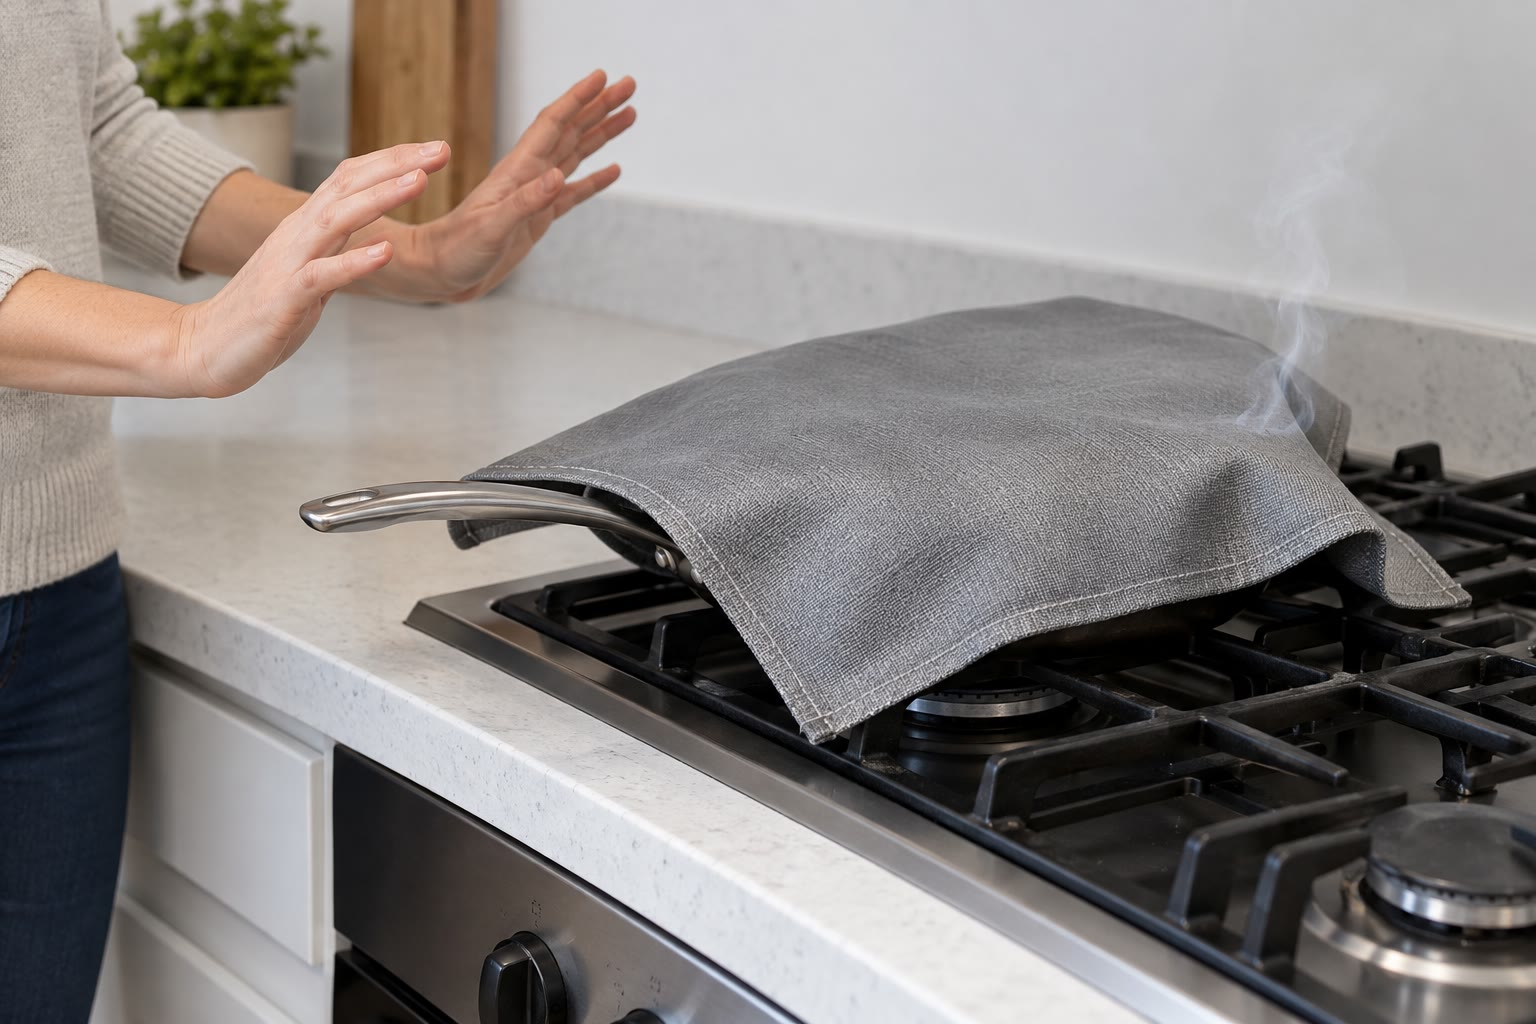
\includegraphics[width=\linewidth,height=4.6cm,keepaspectratio]{images/book1/ai/g4-fire-blanket.jpg}

{\small Une couverture anti-feu sur une poêle~: l'\omterm{def:g4:air-a-mixture-of-gases:air}{air} ne peut plus
atteindre le feu.}
\end{minipage}\hfill
\begin{minipage}[t]{0.48\linewidth}\centering
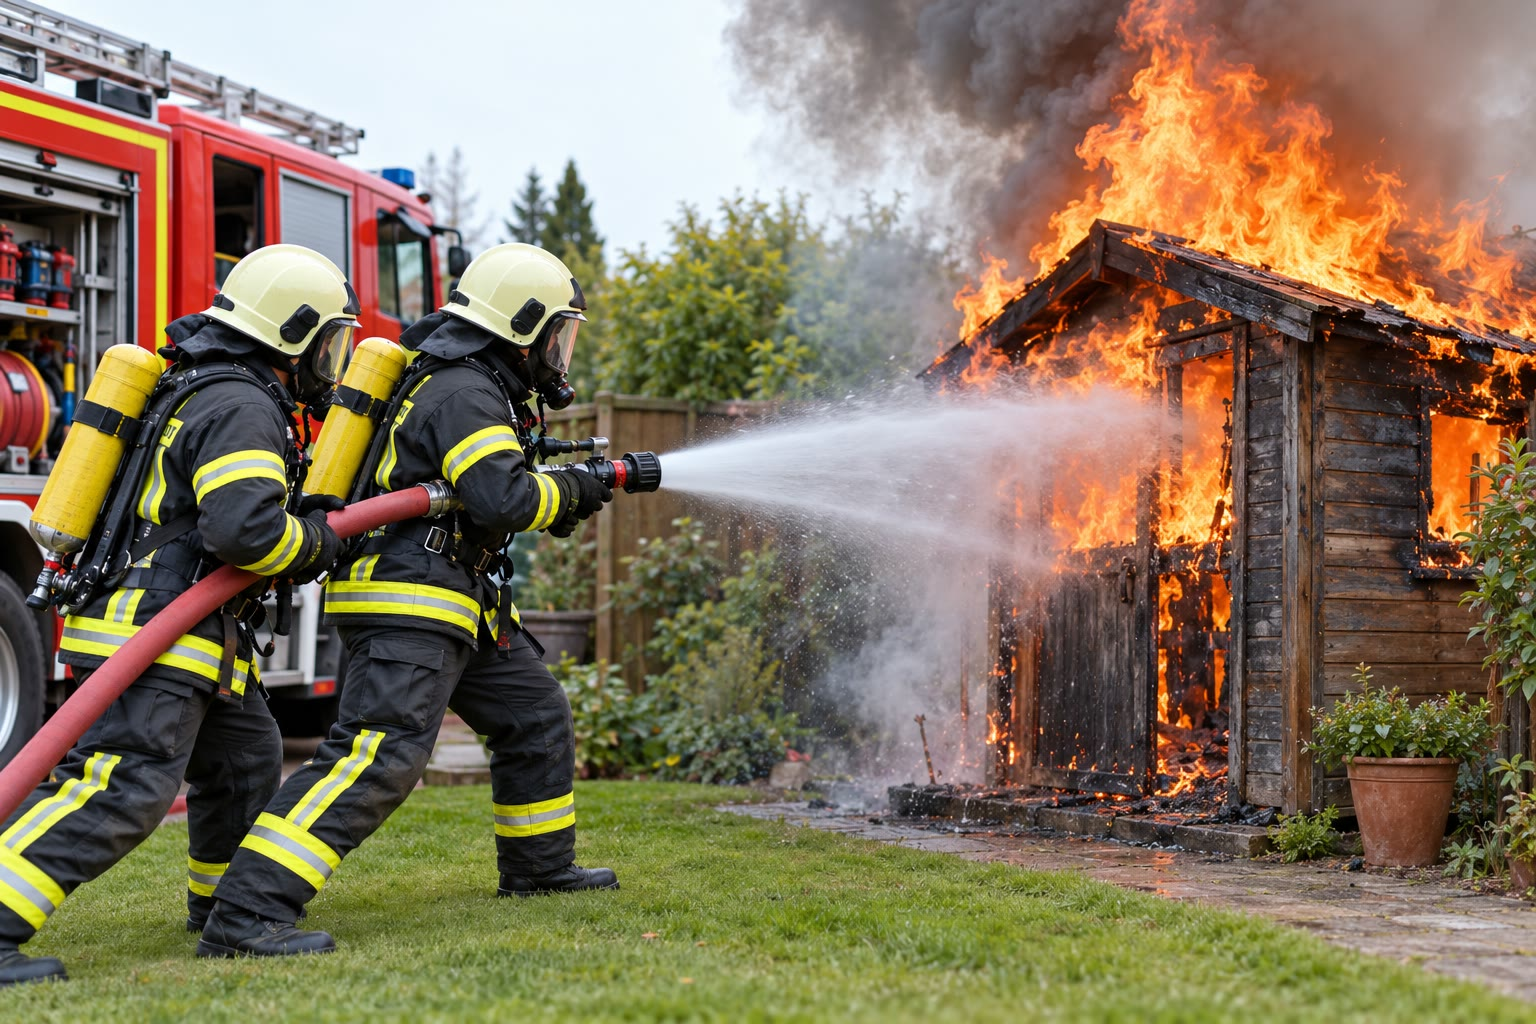
\includegraphics[width=\linewidth,height=4.6cm,keepaspectratio]{images/book1/ai/g4-firefighters.jpg}

{\small Des pompiers arrosent d'eau une cabane en feu pour la refroidir.}
\end{minipage}
\end{omfigure}

\section{La sécurité face au feu}

\begin{remark}[Jamais d'eau sur une poêle d'huile en feu]\label{rem:g4:what-a-fire-needs:oil}
Si l'huile d'une poêle prend feu, il ne faut surtout pas jeter d'eau
dessus~: l'eau bout aussitôt sous l'huile et projette de l'huile en feu
hors de la poêle. Un adulte coupe le gaz ou la plaque, et couvre la
poêle avec un couvercle ou une couverture anti-feu.
\end{remark}

\begin{safety}{\ghs{GHS02}\ghs{GHS04}}
% ledger: ghs:butane
Le gaz d'un briquet ou d'une cartouche de camping est du butane. Son
pictogramme en forme de flamme (GHS02) signifie~: extrêmement
inflammable, tenir à l'écart des flammes et des étincelles. Le
pictogramme en forme de bouteille de gaz (GHS04) signifie~: un gaz
conservé sous pression.
\end{safety}

\begin{proposition}[Que faire en cas d'incendie]\label{prop:g4:what-a-fire-needs:safety}
La fumée est le premier danger d'un incendie~: elle est chaude, elle
cache la sortie et elle est toxique à respirer. Un détecteur de fumée
fixé au plafond sonne très fort dès que la fumée l'atteint. En cas
d'incendie~: sors, baisse-toi sous la fumée, ferme les portes derrière
toi, et appelle les pompiers une fois dehors. Ne rentre jamais.
\end{proposition}

\begin{omfigure}
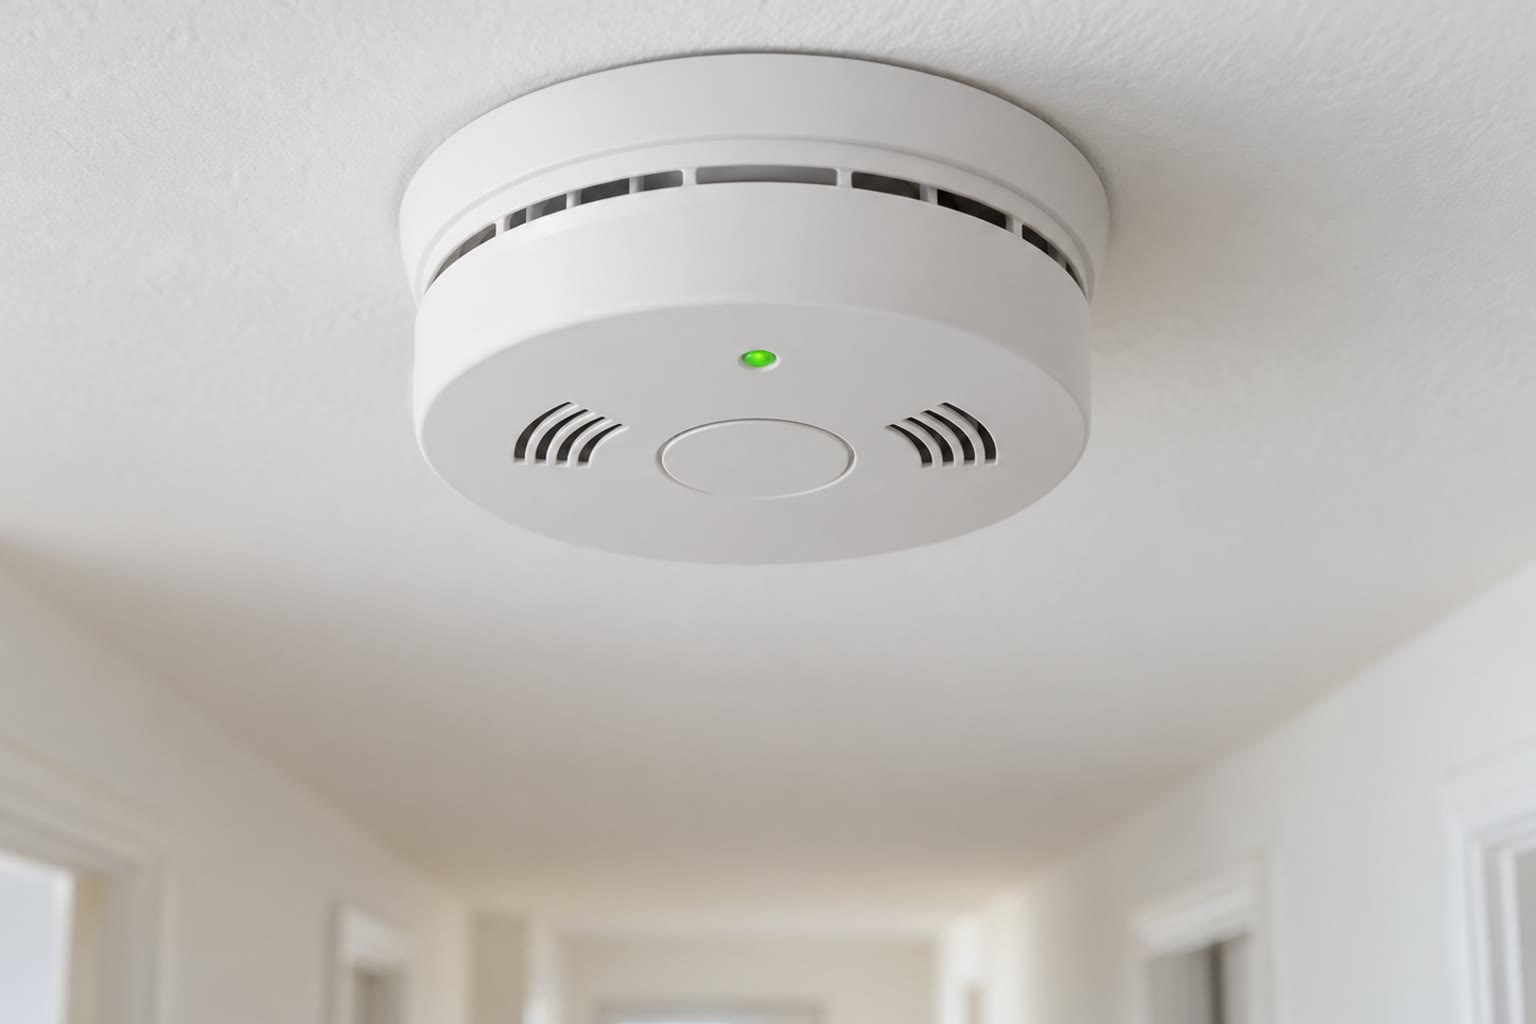
\includegraphics[width=0.42\linewidth]{images/book1/ai/g4-smoke-alarm.jpg}

{\small Un détecteur de fumée~: il sonne dès que la fumée l'atteint.}
\end{omfigure}

\section{Exercices}

\begin{exercise}[$\star$]\label{exo:g4:what-a-fire-needs:1}
Nomme les trois côtés du \omterm{def:g4:what-a-fire-needs:fire-triangle}{triangle du feu}.
\end{exercise}

\begin{exercise}[$\star$]\label{exo:g4:what-a-fire-needs:2}
Lesquels de ces matériaux sont des \omterm{def:g4:what-a-fire-needs:fuel}{combustibles}~: le bois, le sable, la
cire de bougie, le verre, l'essence, l'eau, le papier~?
\end{exercise}

\begin{exercise}[$\star$]\label{exo:g4:what-a-fire-needs:3}
On jette une couverture anti-feu sur un petit feu. Quel côté du
\omterm{def:g4:what-a-fire-needs:fire-triangle}{triangle du feu} enlève-t-elle~?
\end{exercise}

\begin{exercise}[$\star$]\label{exo:g4:what-a-fire-needs:4}
Des pompiers arrosent d'eau une cabane en feu. Quel côté du \omterm{def:g4:what-a-fire-needs:fire-triangle}{triangle du
feu} l'eau enlève-t-elle~?
\end{exercise}

\begin{exercise}[$\star$]\label{exo:g4:what-a-fire-needs:5}
Nomme trois nouvelles substances fabriquées quand le bois \omterm{def:g4:what-a-fire-needs:burning}{brûle}.
\end{exercise}

\begin{exercise}[$\star$]\label{exo:g4:what-a-fire-needs:6}
Pourquoi des braises rougeoyantes se rallument-elles quand on souffle
dessus~?
\end{exercise}

\begin{exercise}[$\star$]\label{exo:g4:what-a-fire-needs:7}
Un verre froid tenu au-dessus d'une bougie se couvre de buée. Quelle
nouvelle substance la bougie a-t-elle fabriquée~?
\end{exercise}

\begin{exercise}[$\star$]\label{exo:g4:what-a-fire-needs:8}
Que dois-tu faire en premier si un détecteur de fumée se déclenche et
que tu vois de la fumée~?
\end{exercise}

\begin{exercise}[$\star$]\label{exo:g4:what-a-fire-needs:9}
Regarde la figure aux trois petits triangles. Quel côté est barré quand
on ferme le gaz~?
\end{exercise}

\begin{exercise}[$\star\star$]\label{exo:g4:what-a-fire-needs:10}
Pour arrêter un feu de forêt, les pompiers abattent parfois une large
bande d'arbres devant lui. Quel côté du \omterm{def:g4:what-a-fire-needs:fire-triangle}{triangle du feu} enlèvent-ils~?
\end{exercise}

\begin{exercise}[$\star\star$]\label{exo:g4:what-a-fire-needs:11}
Une bûche pèse beaucoup plus lourd que sa cendre. Une partie de la bûche
a-t-elle disparu~? Explique où elle est passée.
\end{exercise}
